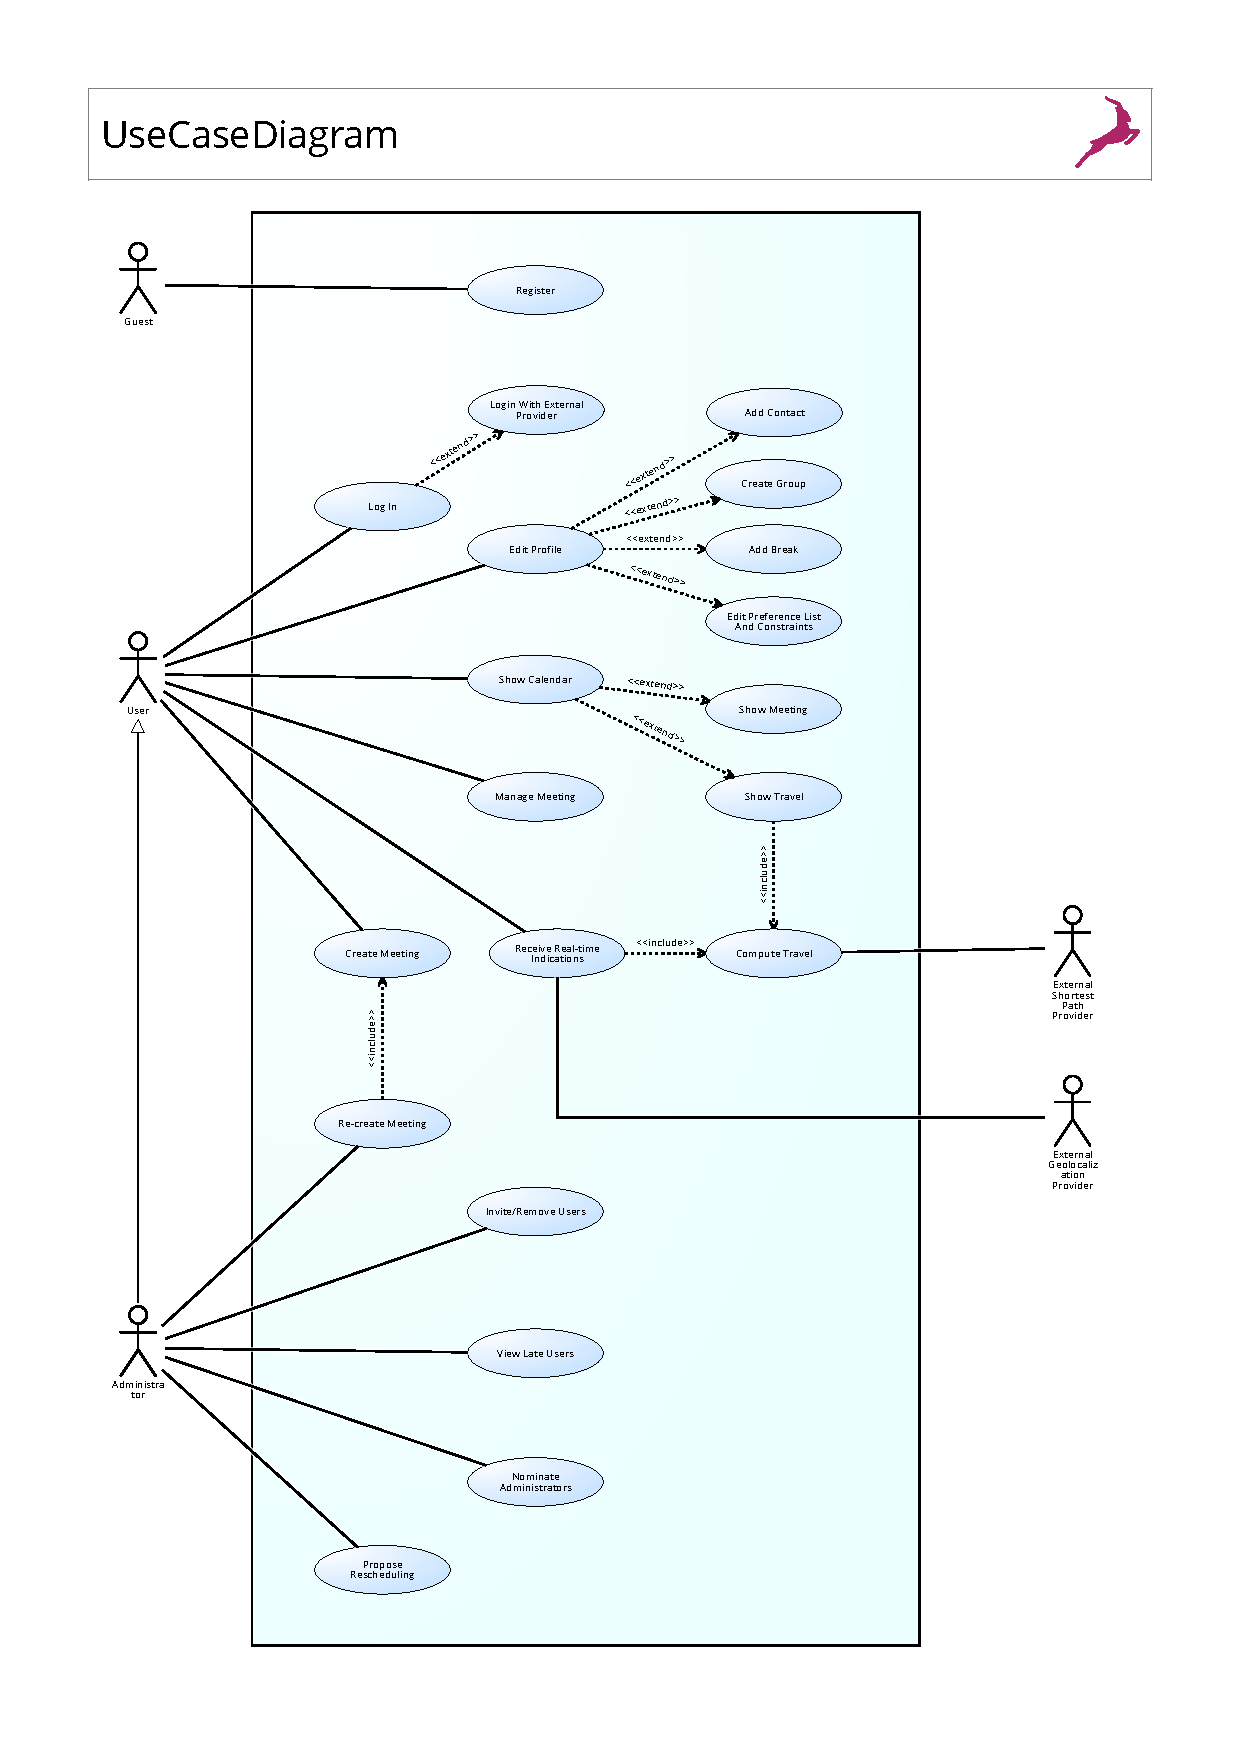
\includepdf[pages=-]{Pdf/UseCaseDiagram.pdf}

\begin{table}[H]
	\centering
	\def\arraystretch{1.5}
	\begin{tabular}{|p{7cm}|p{7cm}|}
		\hline
		\textbf{Actors}            & Guest		    \\ \hline
		\textbf{Goals}             &            \\ \hline
		\textbf{Input Conditions}  &            \\ \hline
		\textbf{Events Flow}       &            \\ \hline
		\textbf{Output Conditions} &            \\ \hline
		\textbf{Exceptions}        &            \\ \hline
	\end{tabular}
	\caption{Register}
\end{table}

\begin{table}[H]
	\centering
	\def\arraystretch{1.5}
	\begin{tabular}{|p{7cm}|p{7cm}|}
		\hline
		\textbf{Actors}            & User		    \\ \hline
		\textbf{Goals}             &            \\ \hline
		\textbf{Input Conditions}  &            \\ \hline
		\textbf{Events Flow}       &            \\ \hline
		\textbf{Output Conditions} &            \\ \hline
		\textbf{Exceptions}        &            \\ \hline
	\end{tabular}
	\caption{Login}
\end{table}

\begin{table}[H]
	\centering
	\def\arraystretch{1.5}
	\begin{tabular}{|p{7cm}|p{7cm}|}
		\hline
		\textbf{Actors}            & User		    \\ \hline
		\textbf{Goals}             &            \\ \hline
		\textbf{Input Conditions}  &            \\ \hline
		\textbf{Events Flow}       &            \\ \hline
		\textbf{Output Conditions} &            \\ \hline
		\textbf{Exceptions}        &            \\ \hline
	\end{tabular}
	\caption{Edit Profile}
\end{table}

\begin{table}[H]
	\centering
	\def\arraystretch{1.5}
	\begin{tabular}{|p{7cm}|p{7cm}|}
		\hline
		\textbf{Actors}            & User		    \\ \hline
		\textbf{Goals}             &            \\ \hline
		\textbf{Input Conditions}  &            \\ \hline
		\textbf{Events Flow}       &            \\ \hline
		\textbf{Output Conditions} &            \\ \hline
		\textbf{Exceptions}        &            \\ \hline
	\end{tabular}
	\caption{Show Calendar}
\end{table}

\begin{table}[H]
	\centering
	\def\arraystretch{1.5}
	\begin{tabular}{|p{7cm}|p{7cm}|}
		\hline
		\textbf{Actors}            & User		    \\ \hline
		\textbf{Goals}             &            \\ \hline
		\textbf{Input Conditions}  &            \\ \hline
		\textbf{Events Flow}       &            \\ \hline
		\textbf{Output Conditions} &            \\ \hline
		\textbf{Exceptions}        &            \\ \hline
	\end{tabular}
	\caption{Manage Meetings}
\end{table}

\begin{table}[H]
	\centering
	\def\arraystretch{1.5}
	\begin{tabular}{|p{7cm}|p{7cm}|}
		\hline
		\textbf{Actors}            & User, External Geolocalization Provider		    \\ \hline
		\textbf{Goals}             &            \\ \hline
		\textbf{Input Conditions}  &            \\ \hline
		\textbf{Events Flow}       &            \\ \hline
		\textbf{Output Conditions} &            \\ \hline
		\textbf{Exceptions}        &            \\ \hline
	\end{tabular}
	\caption{Receive Real-Time Indications}
\end{table}

\begin{table}[H]
	\centering
	\def\arraystretch{1.5}
	\begin{tabular}{|p{7cm}|p{7cm}|}
		\hline
		\textbf{Actors}            & User		    \\ \hline
		\textbf{Goals}             &            \\ \hline
		\textbf{Input Conditions}  &            \\ \hline
		\textbf{Events Flow}       &            \\ \hline
		\textbf{Output Conditions} &            \\ \hline
		\textbf{Exceptions}        &            \\ \hline
	\end{tabular}
	\caption{Create Meeting}
\end{table}

\begin{table}[H]
	\centering
	\def\arraystretch{1.5}
	\begin{tabular}{|p{7cm}|p{7cm}|}
		\hline
		\textbf{Actors}            & Administrator    \\ \hline
		\textbf{Goals}             &            \\ \hline
		\textbf{Input Conditions}  &            \\ \hline
		\textbf{Events Flow}       &            \\ \hline
		\textbf{Output Conditions} &            \\ \hline
		\textbf{Exceptions}        &            \\ \hline
	\end{tabular}
	\caption{Recreate Meeting}
\end{table}

\begin{table}[H]
	\centering
	\def\arraystretch{1.5}
	\begin{tabular}{|p{7cm}|p{7cm}|}
		\hline
		\textbf{Actors}            & Administrator    \\ \hline
		\textbf{Goals}             &            \\ \hline
		\textbf{Input Conditions}  &            \\ \hline
		\textbf{Events Flow}       &            \\ \hline
		\textbf{Output Conditions} &            \\ \hline
		\textbf{Exceptions}        &            \\ \hline
	\end{tabular}
	\caption{Invite/Remove Users}
\end{table}

\begin{table}[H]
	\centering
	\def\arraystretch{1.5}
	\begin{tabular}{|p{7cm}|p{7cm}|}
		\hline
		\textbf{Actors}            & Administrator    \\ \hline
		\textbf{Goals}             &            \\ \hline
		\textbf{Input Conditions}  &            \\ \hline
		\textbf{Events Flow}       &            \\ \hline
		\textbf{Output Conditions} &            \\ \hline
		\textbf{Exceptions}        &            \\ \hline
	\end{tabular}
	\caption{View Late Users}
\end{table}

\begin{table}[H]
	\centering
	\def\arraystretch{1.5}
	\begin{tabular}{|p{7cm}|p{7cm}|}
		\hline
		\textbf{Actors}            & Administrator    \\ \hline
		\textbf{Goals}             &            \\ \hline
		\textbf{Input Conditions}  &            \\ \hline
		\textbf{Events Flow}       &            \\ \hline
		\textbf{Output Conditions} &            \\ \hline
		\textbf{Exceptions}        &            \\ \hline
	\end{tabular}
	\caption{Nominate Administrators}
\end{table}

\begin{table}[H]
	\centering
	\def\arraystretch{1.5}
	\begin{tabular}{|p{7cm}|p{7cm}|}
		\hline
		\textbf{Actors}            & Administrator    \\ \hline
		\textbf{Goals}             &            \\ \hline
		\textbf{Input Conditions}  &            \\ \hline
		\textbf{Events Flow}       &            \\ \hline
		\textbf{Output Conditions} &            \\ \hline
		\textbf{Exceptions}        &            \\ \hline
	\end{tabular}
	\caption{Propose Rescheduling}
\end{table}